% LLNL

\begin{frame}[ctb!]
\frametitle{LLNL Model : Background}
The analytical  model
\begin{itemize} 
  \item was created at LLNL (H. Greenberg, J. Blink, et. al) \cite{hardin_generic_2011, sutton_investigations_2011, 
greenberg_application_2012}
  \item employs an analytic model from Carslaw and Jaeger \cite{carslaw_conduction_1959} 
  \item is implemented in MathCAD \cite{ptc_mathcad_2010}
  \item seeks to inform heat limited waste capacity calculations for 
    \begin{itemize}
      \item arbitrary geology 
      \item arbitrary waste package loading densities
      \item arbitrary homogeneous decay heat source
    \end{itemize}
\end{itemize}
\end{frame}

\begin{frame}
  \frametitle{LLNL Model : Geometry}
  \begin{figure}[h!]
    \begin{center}
      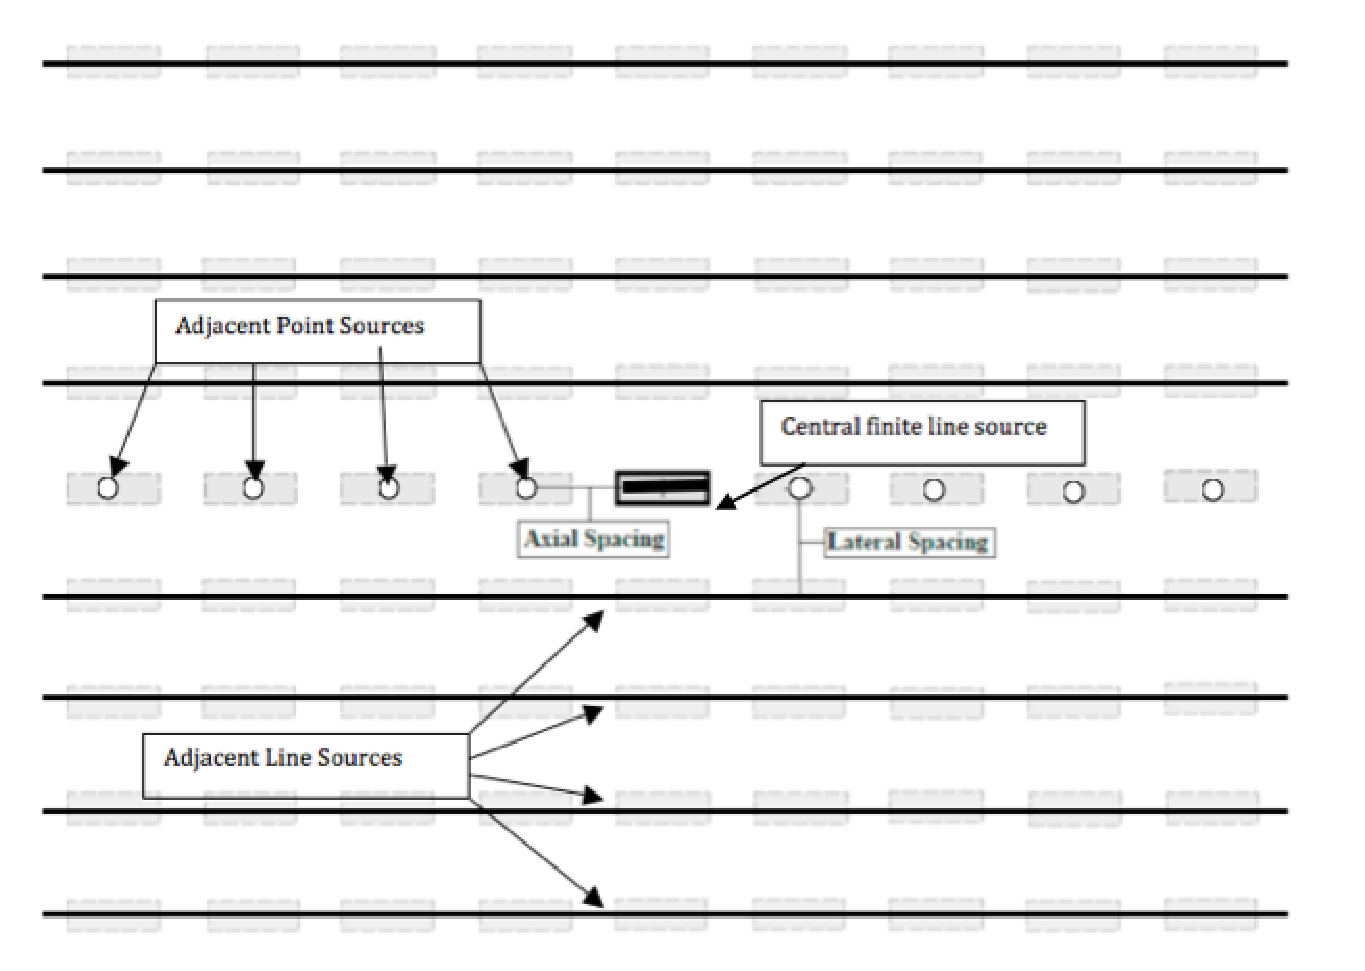
\includegraphics[width=0.7\columnwidth]{images/llnlConcept.eps}
    \end{center}
    \caption{Vertical, horizontal, alcove, and borehole emplacement layouts can 
    be represented by a line of point sources and adjacent line sources 
    \cite{sutton_investigations_2011}.}
    \label{fig:llnl}
  \end{figure}
\end{frame}

